\documentclass{article}
\usepackage{epsfig}

\newcommand{\skewstart}{%
  \ensuremath{\sigma_\mathrm{start}}}

\newcommand{\skewend}{%
  \ensuremath{\sigma_\mathrm{end}}}

\begin{document}

\title{Transformations to and from Track Coordinates in Vamos}
\author{Sam Varner\\ \texttt{snick-a-doo@comcast.net}}
\maketitle

This document describes in detail the coordinate transformations that
go on when dealing with tracks in Vamos.  I it in an attempt to
understand some problems with dealing with the skew parameter.

Early on, I made the decision to treat tracks as narrow strips made up
of straight and curved segments rather than mesh surfaces.  A mesh
would allow greater realism, but it would be harder to adjust.  I
don't regret that decision, but I've found that when I need a segment
that's not straight or the arc of a circle (e.g. skewed curves or pit
lanes) the geometry can get tricky.

The figures are from PostScript files generated by Lisp code which
implements the transformations described below.  The angles and
distances are precise, although many of the figures are accidental
optical illusions that make some lines look bent and circles look
squashed. 

\section{Track Coordinates and World Coordinates}

The physics calculations in Vamos are done in a three-dimensional
Cartesian coordinate system referred to as the {\em world
  coordinates}.  The axes of the world coordinates are denoted $x$,
$y$, and $z$, with $z$ being the vertical axis.

Sometimes it is convenient to consider a curvilinear coordinate system
that follows the track.  In these {\em track coordinates}, $q_0$ runs
along the track reference curve---the path defined by the lengths and
radii in the track definition file.  the distance from the reverence
curve is $q_1$.  This coordinate is perpendicular to $q_0$ except in
the presence of skew.  See Section~\ref{section:skew}.  The vertical
dimension is $q_2$, which is the same as the $z$-coordinate in the
world frame.  This coordinate is use to test for contact with the
ground.

When we talk about ``distance along the track'' we mean $q_0$.  It's
used to define the track length and the position of timing lines.  The
coordinate $q_1$ is used to determine if a point is on the track, on
the shoulder, or in contact with the wall.

\section{From Track Coordinates to World Coordinates}

The track is specified as a set of adjoining straight and curved
segments.  The lengths of the segments are distances in $q_0$; the
widths are distances in $q_1$.  So, rendering the track in world
coordinates involves a transformation from track coordinates.

\subsection{Without Skew}

When there is no skew, the transformation is straightforward.  For a
straight segment
\begin{eqnarray}
  \label{eq:straight-to-world}
  x & = & x_0 + d \cos \theta - q_1 \sin \theta \\
  y & = & y_0 + d \sin \theta + q_1 \cos \theta \nonumber
\end{eqnarray}
where $x_0$ and $y_0$ are the world coordinates at the end of the
previous segment, $d$ is the distance from the start of the segment
and $\theta$ is the angle with respect to the world $x$-axis.  For the
first segment, $x_0 = y_0 = 0$ and, unless otherwise
specified by the \verb/<start-direction>/ tag in the track definition
file, $\theta = 0$.

For a curved segment with no skew,
\begin{eqnarray}
  \label{eq:curve-to-world}
  x & = & x_c + (r - q_1) \sin (\theta + \alpha) \\
  y & = & y_c - (r - q_1) \cos (\theta + \alpha) \nonumber
\end{eqnarray}
where $x_c$ and $y_c$ are the coordinates of the center of curvature
\begin{eqnarray}
  \label{eq:center}
  x_c & = & x_0 - r \sin \theta \\ 
  y_c & = & y_0 + r \cos \theta \nonumber
\end{eqnarray}
and $\alpha = d/r$.  Left turns have positive radii; right turns have
negative radii.

\subsection{With Skew}
\label{section:skew}

If a curve is very sharp, the segments before and after the curve may
overlap. (See Figure~\ref{fig:overlap}a.)  As a result, part of the
barrier for the segment leaving the curve may appear to block the
segment entering the curve.  (In actuality, a car will not actually
run into such a wall because it is not part of the car's current
segment.)

\begin{figure}
  \centering
  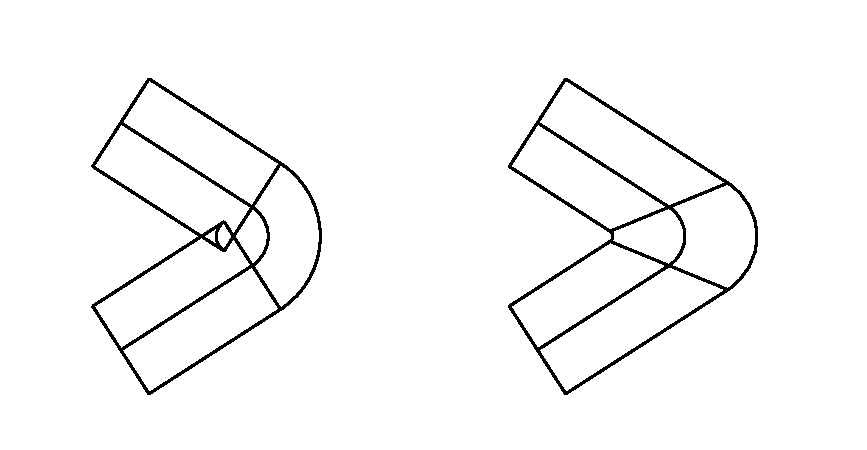
\epsfig{file=overlap.eps, width=10cm}
  \caption{The effect of skew on a tight 2-radian turn where the width
    of the track is three times the radius of the reference line.
    Overlap of the entering and exiting straight segments can be seen
    in (a) where $\sigma = 0$.  In (b) $\sigma = 0.7$; all other
    parameters are unchanged.}
  \label{fig:overlap}
\end{figure}

To avoid such artifacts, curves can be distorted so that adjacent
segments do not overlap.  The distortion is called {\em skew} because
it causes the $q_1$ dimension to become slanted so that it's not
perpendicular to $q_0$.  The skew parameter, $\sigma$, is defined by
\begin{equation}
  \label{eq:skew-definition}
  \sigma \equiv dq_0/dq_1
\end{equation}
measured at the beginning of a segment.  For a skewed curve, the
boundaries of the segment do not pass through the center of curvature.
Consequently, the arcs of constant $q_1$ are not concentric, as can be
seen in Figure~\ref{fig:overlap}b.  Note that the centerline of the
track is unchanged by the skew.

When a segment is skewed, adjoining segments must also be skewed so
that there's not a gap.  But we have to make sure the skew stops
propagating somewhere.  Skew is always applied symmetrically to curved
segments, simply to keep the math from getting out of hand.  The math
for straight segments is easier, so we can allow straight segments
that are skewed at one end and not the other.

Here are the rules for propagating skew
\begin{itemize}
\item Skew may be specified only for curves.
\item The skew at the end of the curve is the negative of the skew at
  the start.
\item The ends of straight segments are automatically skewed to match
  the segments they connect to.
\item A curved segment that follows a skewed curve is skewed
  (symmetrically) to match.
\item The beginning and end of a track are not skewed.
\end{itemize}

The transformation from a skewed straight segment to world coordinates
is the same as Equation~\ref{eq:straight-to-world} with $q_0$ modified
by a linear transformation.
\begin{eqnarray}
  \label{eq:skewed-straight-to-world}
  x & = & x_0 + d^\prime \cos \theta - q_1 \sin \theta \\
  y & = & y_0 + d^\prime \sin \theta + q_1 \cos \theta \nonumber
\end{eqnarray}
where 
\begin{equation}
 \label{eq:d-prime}
  d^\prime =  q_1 \skewstart + d(1 + q_1\Delta\sigma/l).
\end{equation}
Here, $l$ is the length of the segment, and $\Delta\sigma = \skewend -
\skewstart$.  The effect of skew on a
straight segment is shown in Figure~\ref{fig:straight}.

\begin{figure}
  \centering
  \epsfig{file=straight.eps, width=8cm}
  \caption{Unskewed and skewed straight segments with lines of
    constant $q_0$ and $q_1$.  The skewed segment has $\sigma=0.4$ on
    the left and $\sigma=-0.8$ on the right.}
  \label{fig:straight}
\end{figure}

For skewed curves, the $r$, $x_c$, and $y_c$ in
Equation~\ref{eq:curve-to-world} become linear functions of $q_1$.
\begin{eqnarray}
  x & = & x_c^\prime + (r^\prime - q_1) \sin (\theta + \alpha) \\
  y & = & y_c^\prime - (r^\prime - q_1) \cos (\theta + \alpha) \nonumber
\end{eqnarray}
with
\begin{eqnarray}
  \label{eq:curve-primes}
  r^\prime & = & 
  r - q_1 \frac{\skewstart}{\tan\beta} \\
  x_c^\prime & = & 
  x_c + q_1 \skewstart \frac{\sin (\theta + \beta)}{\sin\beta}
  \nonumber \\
  y_c^\prime & = & 
  y_c - q_1 \skewstart \frac{\cos (\theta + \beta)}{\sin\beta}
  \nonumber
\end{eqnarray}
where $\beta \equiv \Delta \alpha / 2$; half the angle subtended by
the curve, and $x_c$ and $y_c$ are as defined in
Equation~\ref{eq:center}.  The effect of skew on a curved segment is
shown in Figure~\ref{fig:curve}.  For right turns, $\alpha$ is
negative.

\begin{figure}
  \centering
  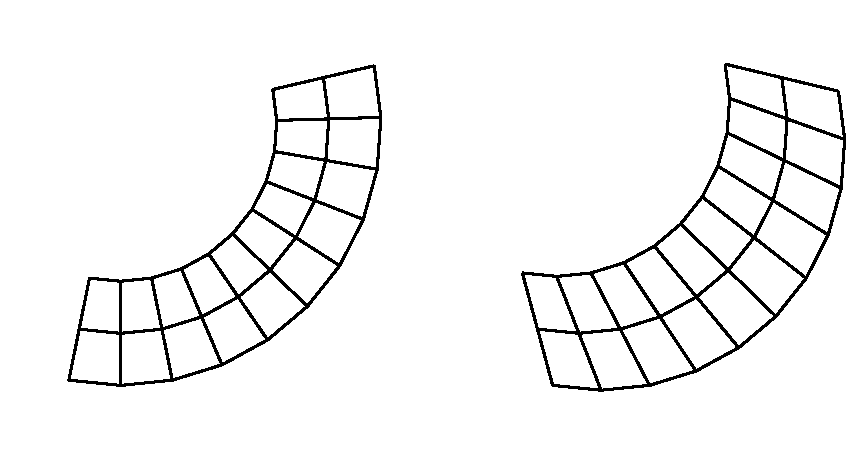
\epsfig{file=curve.eps, width=8cm}
  \caption{Unskewed and skewed curved segments with lines of
    constant $q_0$ and $q_1$.  The skewed segment has $\sigma=-0.5$.}
  \label{fig:curve}
\end{figure}

\section{From World Coordinates to Track Coordinates}

To find out when a car crosses the finish line or a timing line, we
need to transform its Cartesian coordinates to $q_0$.  And to find out
if it's on the track or if it has run into the wall we need $q_1$.

The equations from the previous sections are readily solved for
$d^\prime$, $\alpha$, and $q_1$:
\begin{eqnarray}
  d^\prime & = & (x - x_0)\cos\theta - (y - y_0)\sin\theta \\
  q_1 & = & (x - x_0)\sin\theta + (y - y_0)\cos\theta \nonumber
\end{eqnarray}
for straights, and
\begin{eqnarray}
  \label{eq:curve-to-track}
  \alpha & = & \tan\left(\frac{y - y_c^\prime}{x - x_c^\prime}\right) + \beta \\
  q_1 & = & r^\prime - \sqrt{(x - x_c^\prime)^2 + (y - y_c^\prime)^2} \nonumber
\end{eqnarray}
for curves.  Since a right turn has a negative radius, we need to add
$\pi$ to $\alpha$.  In the code, where the tangent is computed by
\verb/atan2(y, x)/ it's convenient to change the sign of the arguments
so that $-\pi < \alpha \leq \pi$.

When a straight is skewed, $q_1$ is unchanged, but $d$ becomes
$d^\prime$ as in Equation~\ref{eq:d-prime}.  Solving for $d^\prime$
gives
\begin{equation}
  d = \frac{d^\prime - q_1 \skewstart}{1 + q_1\Delta\sigma/l}.
\end{equation}

For a skewed curve, we substitute Equations~\ref{eq:curve-primes} into
Equation~\ref{eq:curve-to-track}.  This is much easier if we transform
to a coordinate system with its origin at $(x_c, y_c)$ oriented so
that the $x$-axis bisects the curve.  In this case $x_c^\prime = q_1
\skewstart / sin\beta$, $y_c^\prime = 0$.  After substitution and
collecting terms we have
\begin{equation}
  \label{eq:q1-solution}
  q_1^2\left(\sigma^2 - \frac{2\sigma}{\tan\beta} - 1\right) 
  + 2q_1\left(\frac{\sigma}{\sin\beta}(r\cos\beta - x) + r \right)
    + x^2 + y^2 - r^2 = 0
\end{equation}
which we can solve with the quadratic formula\ldots if we're careful.

We have terms that blow up for arcs that are zero or multiples of 360
degrees.  A zero-degree turn has no length and will be ignored when
the track is read in.  There is no special protection against
360-degree turns; you'll just get a math error.  If you really want a
360-degree turn, use two 180s. 

We also have to check to see if the coefficient on the squared term is
zero.  If that's the case then it's easy to solve the linear equation
for $q_1$, but trying to use the quadratic formula will result in
division by zero.

Now, we still need to decide which root to pick when the $q_1^2$ term
is present, and we need to decide what to do if the roots are complex.
Some pictures will help us decide.

Equation~\ref{eq:curve-to-track} shows that lines of constant $q_1$
are circles.  So, solving for $q_1$ is the same as finding the circle
that goes through the given $(x, y)$ point.  Figure~\ref{fig:circles}
shows lines of constant $q_1$ for a two-radian turn with various
skews.  

\begin{figure}
  \centering
  \epsfig{file=circles.eps, width=8cm}
  \caption{Lines of constant $q_1$ for a two-radian turn.  The skews
    are (from left to right, top to bottom): 0, -0.3, $-\pi/6$
    ($\approx -0.524$), -1, $-\pi/2$ ($\approx -1.57$), and 0.5.}
  \label{fig:circles}
\end{figure}

I don't have an interpretation for the two roots of
Equation~\ref{eq:q1-solution}.  Looking at the numbers, it's clear
that the smaller root is appropriate for left turns, and the larger is
for right turns.  

Complex roots occur for points outside of the family of constant-$q_1$
circles.  The third, fourth, and fifth diagrams in
Figure~\ref{fig:circles} have regions where complex roots occur.  Even
in these cases, complex roots are rare in practice because the track
segment ends inside the region of real solutions.  In the event that a
complex root is found when transitioning to the next segment, the
$y$-coordinate can be used to determine whether we've gone off the
beginning or the end of the segment.

\begin{figure}
  \centering
\begin{verbatim}
(defmacro with-ps-file (stream file &body body)
  "Send PostStript commands to FILE and insert the obligatory lines.
The file is suitable for including in a LaTeX document, although
the bounding box might have to be adjusted."
  `(with-open-file (,stream ,file
                            :direction :output
                            :if-exists :supersede)
     (format stream "%!PS-Adobe-3.0 EPSF-3.0~%")
     (format stream "%%BoundingBox: 0 0 400 200~%")
     ,@body
     (format ,stream "~&showpage~%")))

(defun ps-line (stream xy1 xy2)
  "Print the PostStript code for drawing a line.
xy1 and xy2 are cons cells."
  (format stream "~&~F ~F moveto~%" (car xy1) (cdr xy1))
  (format stream "~F ~F lineto~%" (car xy2) (cdr xy2))
  (format stream "stroke~%"))

(defun ps-arc (stream xc yc radius angle arc)
  "Print the PostStript code for drawing an arc."
  (labels ((rad->deg (angle) 
             (- (* angle (/ 180 pi))
                90)))
    (format stream "~F ~F ~F ~F ~F arc~%" 
            xc yc radius
            (rad->deg angle)
            (rad->deg (+ angle arc)))
    (format stream "stroke~%")))
\end{verbatim}
  \caption{PostScript-generating functions}
\end{figure}

\begin{figure}
  \centering
\begin{verbatim}
(defun straight (d q1 x0 y0 theta l sigma-start sigma-end)
  "Return the world coordinates for track coordinates D and Q1 on a
straight segment."
  (let ((d-prime (+ (* d (1+ (* q1 (/ (- sigma-end sigma-start) l))))
                    (* q1 sigma-start))))
    (cons (+ x0 
             (* d-prime (cos theta)) 
             (* (- q1) (sin theta)))
          (+ y0
             (* d-prime (sin theta))
             (* q1 (cos theta))))))

(defun r-prime (r q1 sigma beta)
  "Return the radius of a skewed curve."
  (- r (* q1 (/ sigma (tan beta)))))

(defun xc-prime (xc q1 sigma theta beta)
  "Return the x-coordinate for the center of a skewed curve."
  (+ xc (* q1 sigma (/ (sin (+ theta beta))
                       (sin beta)))))

(defun yc-prime (yc q1 sigma theta beta)
  "Return the y-coordinate for the center of a skewed curve."
  (- yc (* q1 sigma (/ (cos (+ theta beta))
                       (sin beta)))))

(defun curve (alpha q1 x0 y0 theta r arc sigma-start)
  "Return the world coordinates for track coordinates ALHPA and Q1 on
a cuved segment."
  (let* ((xc (- x0 (* r (sin theta))))
         (yc (+ y0 (* r (cos theta))))
         (beta (/ arc 2))
         (radius (- (r-prime r q1 sigma-start beta) q1)))
    (cons (+ (xc-prime xc q1 sigma-start theta beta)
             (* radius (sin (+ theta alpha))))
          (- (yc-prime yc q1 sigma-start theta beta) 
             (* radius (cos (+ theta alpha)))))))
\end{verbatim}
\caption{Implementation of equations in the text}
\end{figure}

\begin{figure}
  \centering
\begin{verbatim}
(defun solve-quadratic (a b c)
  "Solve a quadratic (or linear) equation of the form 
Ax^2 + Bx + C = 0."
  (if (zerop a)
      (- (/ c b))
      (let ((discriminant (- (* b b) (* 4 a c))))
        (values (/ (+ (- b) (sqrt discriminant)) (* 2 a))
                (/ (- (- b) (sqrt discriminant)) (* 2 a))))))

(defun solve-for-q1 (x y radius arc skew)
  "Return the track coordinate Q1 for world coordinates (X, Y) on a
skewed curve."
  (let ((beta (/ arc 2)))
    (multiple-value-bind (q1+ q1-)
        (solve-quadratic
         (+ (* skew skew) 
            (/ (* -2 skew) (tan beta)) 
            -1)
         (* 2 (+ (* (/ skew (sin beta))
                    (- (* radius (cos beta)) x))
                 radius))
         (+ (* x x) 
            (* y y)
            (- (* radius radius))))
      (if (plusp radius) q1- q1+))))

(defun alpha (x xc y yc arc)
  "Return the angle traveled through the curve for world
coordinates (X, Y) on skewed curve."
    (+ (atan (* (- y yc) (signum arc))
             (* (- x xc) (signum arc)))
       (/ arc 2)))
\end{verbatim}
\caption{Implementation of equations in the text (continued)}
\end{figure}

\begin{figure}
  \centering
\begin{verbatim}
(defmacro do-range ((value start range steps) &body body)
  "Loop over a range."
  (let ((count (gensym))
        (increment (gensym))
        (g-steps (gensym)))
    `(let* ((,g-steps ,steps)
            (,increment (/ ,range (- ,g-steps 1))))
       (do ((,count 0 (+ ,count 1))
            (,value ,start (+ ,value ,increment)))
           ((= ,count ,g-steps))
         ,@body))))

(defmacro do-lines (((x next-x x-start x-range x-steps)
                     (y next-y y-start y-range y-steps))
                    &body body)
  "Loop over a grid setting X, Y, NEXT-X, NEXT-Y to grid points.
Drawing lines between each (X, Y) and (NEXT-X, NEXT-Y) point results
in a set of lines of constant y-value in the x-dimension."
  (let ((x-count (gensym)) (x-interval (gensym)) 
        (g-x-start (gensym)) (g-x-steps (gensym))
        (y-count (gensym)) (y-interval (gensym)) (g-y-steps (gensym)))
    `(let ((,g-x-start ,x-start)
           (,g-x-steps ,x-steps)
           (,g-y-steps ,y-steps))
      (do* ((,y-count 0 (+ ,y-count 1))
            (,y-interval (/ ,y-range ,g-y-steps))
            (,y ,y-start (+ ,y ,y-interval))
            (,next-y ,y ,y))
           ((> ,y-count ,g-y-steps))
        (do* ((,x-count 0 (+ ,x-count 1))
              (,x-interval (/ ,x-range ,g-x-steps))
              (,x ,g-x-start ,next-x)
              (,next-x (+ ,g-x-start ,x-interval) (+ ,next-x ,x-interval)))
             ((= ,x-count ,g-x-steps))
          ,@body)))))

(defmacro do-grid ((x-spec y-spec) &body body)
  "Draw a grid.  Each -SPEC is a list of the form (var next-var start
range steps).  Drawing a line between each (x-var, y-var) and
(x-next-var, y-next-var) results in a x-steps by y-steps grid."
  `(progn 
    (do-lines (,x-spec ,y-spec) ,@body)
    (do-lines (,y-spec ,x-spec) ,@body)))
\end{verbatim}
  \caption{Macros used by the figure-drawing functions}
\end{figure}


\begin{figure}
  \centering
\begin{verbatim}
(defun draw-straight (stream x0 y0 angle width length divisions
                             &key (start-skew 0.0) (end-skew 0.0))
  "Draw a straight segment with lines of constant d and q1."
  (do-grid ((d next-d 0 length divisions)
            (q1 next-q1 (/ width -2) width 2))
    (ps-line stream
             (straight d q1 x0 y0 angle length start-skew end-skew)
             (straight next-d next-q1 x0 y0 angle length start-skew end-skew))))

(defun draw-curve (stream x0 y0 start-angle width radius arc divisions
                          &key (skew 0.0))
  "Draw a curved segment with lines of constant d and q1."
  (do-grid ((angle next-angle 0 arc divisions)
            (q1 next-q1 (/ width -2) width 2))
    (ps-line stream
             (curve angle q1 x0 y0 start-angle radius arc skew)
             (curve next-angle next-q1 x0 y0 start-angle radius arc skew))))

(defun draw-arc (stream x0 y0 radius q1 angle arc skew 
                 &optional show-full-circle)
  "Draw an arc of a skewed curve.  If SHOW-FULL-CIRCLE is non-nil the
complete circle is drawn.  Note that ANGLE and ARC are needed for the
skew calculations even if the full circle is drawn."
  (ps-arc stream 
          (xc-prime x0 q1 skew angle (/ arc 2)) 
          (yc-prime y0 q1 skew angle (/ arc 2)) 
          (- (r-prime radius q1 skew (/ arc 2)) q1)
          angle 
          (if show-full-circle 
              (* 2 pi)
              arc)))
\end{verbatim}
\caption{Figure-drawing functions}
\end{figure}

\begin{figure}
  \centering
\begin{verbatim}
(defun draw-corner (stream x0 y0 length width radius arc
                           &key (skew 0.0))
  "Draw a curve with preceeding and following straight segments."
  (let ((angle (/ (- pi arc) 2)))
    (draw-straight stream x0 y0 angle width length 1
                   :end-skew skew)
    (incf x0 (- (* length (cos angle))
                (* radius (sin angle))))
    (incf y0 (+ (* length (sin angle))
                (* radius (cos angle))))
    (do-range (q1 (/ width -2) width 3)
      (draw-arc stream x0 y0 radius q1 angle arc skew))
    (incf angle arc)
    (incf x0 (* radius (sin angle)))
    (decf y0 (* radius (cos angle)))
    (draw-straight stream x0 y0 angle width length 1 
                   :start-skew (- skew))))

(defun draw-circles (stream x0 y0 skew)
  "Draw circles of constant q1 with coordinate axes."
  (let ((size 75)
        (radius 40)
        (width 40))
    (ps-line stream (cons (- x0 size) y0) (cons (+ x0 size) y0))
    (ps-line stream (cons x0 (- y0 size)) (cons x0 (+ y0 size)))
    (do-range (q1 (/ width -2) width 3)
      (draw-arc stream x0 y0 radius q1 (- (/ pi 2) 1) 2 skew 
                :circle))))
\end{verbatim}
\caption{Figure-drawing functions (continued)}
\end{figure}

\begin{figure}
  \centering
\begin{verbatim}
;; Figure 1
(with-ps-file stream "overlap.eps"
  (draw-corner stream 50 40 75 50 (/ 50 3.0) 2)
  (draw-corner stream 250 40 75 50 (/ 50 3.0) 2
                 :skew -0.7))

;; Figure 2
(with-ps-file stream "straight.eps"
  (draw-straight stream 30 50 0.6 50 200 10)
  (draw-straight stream 250 50 0.6 50 200 10 
                 :start-skew 0.4 :end-skew -0.8))

;; Figure 3
(with-ps-file stream "curve.eps"
  (draw-curve stream 30 50 -0.2 50 100 2 10)
  (draw-curve stream 250 50 -0.2 50 100 2 10
              :skew -0.5))

;; Figure 4
(with-ps-file stream "circles.eps"
  (draw-circles stream 30 250 0)
  (draw-circles stream 200 250 -0.3)
  (draw-circles stream 370 250 (/ pi -6))
  (draw-circles stream 30 50 -1)
  (draw-circles stream 200 50 (- (/ pi 2)))
  (draw-circles stream 370 50 0.5))
\end{verbatim}
\caption{Code used to generate the figures in the text}
\end{figure}

\end{document}
